%% LyX 2.3.6 created this file.  For more info, see http://www.lyx.org/.
%% Do not edit unless you really know what you are doing.
\documentclass[brazil,handout]{beamer}
\usepackage[T1]{fontenc}
\usepackage[utf8]{inputenc}
\usepackage{amssymb}
\usepackage{cancel}
\PassOptionsToPackage{normalem}{ulem}
\usepackage{ulem}

\makeatletter
%%%%%%%%%%%%%%%%%%%%%%%%%%%%%% Textclass specific LaTeX commands.
% this default might be overridden by plain title style
\newcommand\makebeamertitle{\frame{\maketitle}}%
% (ERT) argument for the TOC
\AtBeginDocument{%
  \let\origtableofcontents=\tableofcontents
  \def\tableofcontents{\@ifnextchar[{\origtableofcontents}{\gobbletableofcontents}}
  \def\gobbletableofcontents#1{\origtableofcontents}
}

%%%%%%%%%%%%%%%%%%%%%%%%%%%%%% User specified LaTeX commands.
\usepackage{listings}
\usepackage{listingsutf8}
\lstset{inputencoding=utf8}
% Estilo para blocos de código com fundo escuro
\lstdefinestyle{codeblock}{%
  backgroundcolor=\color{black},
  basicstyle=\ttfamily\footnotesize\color{white},
  keywordstyle=\color{lightblue},
  stringstyle=\color{lightgreen},
  commentstyle=\color{lightred},
  numberstyle=\tiny\color{white},
  numbers=none,
  frame=single,
  rulecolor=\color{white},
  frameround=tttt,
  xleftmargin=0pt,
  framexleftmargin=4pt,
  framexrightmargin=4pt,
  framextopmargin=4pt,
  framexbottommargin=4pt,
  breaklines=false
}
\usepackage{hyperref}
\usepackage{graphicx}
\graphicspath{{./}{../images/}{images/}}

\usepackage{tikz} 
\usetikzlibrary{scopes}

\definecolor{darkred}{rgb}{0.5,0,0}
\definecolor{darkgreen}{rgb}{0,0.5,0}
\definecolor{darkblue}{rgb}{0,0,0.5}

\definecolor{lightred}{rgb}{1,0.8,0.8}
\definecolor{lightgreen}{rgb}{0.8,1,0.8}
\definecolor{lightblue}{rgb}{0.8,0.8,1}

% Caixa colorida para destacar fórmulas
% Macro de caixa destacada solicitada
\newcommand{\cbox}[1]{\begin{center}\Large \fcolorbox{black}{lightred}{#1}\end{center}}

%\usetheme{Warsaw}
% or ...
%\usetheme{Antibes}	% tree outline, neat
%\usetheme{JuanLesPins}	% like Antibes, with shading
%\usetheme{Bergen}	% outline on side
%\usetheme{Luebeck}	% like Warsaw, square sides
%\usetheme{Berkeley}	% interesting left bar outline
%\usetheme{Madrid}	% clean, nice.  7/12 page numbers
%\usetheme{Berlin}	% dots show slide number
%\usetheme{Malmoe}	% OK, plain, unshaded
%\usetheme{Boadilla}	% nice, white bg, no top bar
%\usetheme{Marburg}	% nice, outline on right
%\usetheme{boxes}	% ???
%\usetheme{Montpellier}	% tree outline on top, plainish white
%\usetheme{Copenhagen}	% like Warsaw
%\usetheme{PaloAlto}	% looks good
%\usetheme{Darmstadt}	% like Warsaw with circle outline
%\usetheme{Pittsburgh}
%\usetheme{default}
%\usetheme{Rochester}	% like boxy, unshaded warsaw
%\usetheme{Dresden}	% circle outline on top
%\usetheme{Singapore}	% purple gradient top
%\usetheme{Frankfurt}	% like Warsaw with circle outline on top
%\usetheme{Szeged}
%\usetheme{Goettingen}	% light purple right bar outline
%\usetheme{Warsaw}
%\usetheme{Hannover}	% like Goett with bar on left
%\usetheme{compatibility}
%\usetheme{Ilmenau}

\setbeamercovered{transparent}
% or whatever (possibly just delete it)

%\usecolortheme{seahorse}
\usecolortheme{crane}

% seems to fix typewriter font in outline header:
% Fonte moderna com bom suporte a T1/UTF-8
\usepackage{lmodern}

\usetheme{default} 

%Old themes: bars, boxes, classic, default, lined, plain, shadow, sidebar, sidebardark, sidebardarktab, sidebartab, split, tree, treebars
%New themes (v3.0)
%W/o navigation bar: default, boxes, Bergen, Madrid, Pittsburgh, Rochester
%With a tree-like navigation bar: Antibes, JuanLesPins, Montpellier.
%With a TOC sidebar: Berkeley, PaloAlto, Goettingen, Marburg, Hannover
%With a mini frame navigation: Berlin, Ilmenau, Dresden, Darmstadt, Frankfurt, Singapore, Szeged
%With section and subsection titles: Copenhagen, Luebeck, Malmoe,Warsaw

\makeatother

\usepackage[brazil]{babel}
\begin{document}

% ------------------------------------------------------------------
% Metadados da apresentação
% ------------------------------------------------------------------

\title[Otimização Quântica Híbrida (QAOA) para Problema Simples Inspirado no Posicionamento de Turbinas Eólicas: Uma Prova de Conceito]{Otimização Quântica Híbrida (QAOA) para Problema Simples Inspirado no Posicionamento de Turbinas Eólicas: Uma Prova de Conceito}
% \subtitle{Encontro Potiguar de Física 2025}
\author{Marcos Vinícius Cândido Henriques$^1$}
\institute{$^1$Universidade Federal Rural do Semi-Árido / Campus Angicos}
\date{Martins-RN, 2025}
% Logo do evento no topo do título
\addtobeamertemplate{title page}{%
  \vspace*{0.2cm}
  \begin{center}
    
\includegraphics[height=1.5cm]{logo-evento.jpg}%
  \end{center}
  \vspace{-0.2cm}% espaço abaixo do logo
}{}

\makebeamertitle

\logo{}

% Logo/imagem no rodapé, canto inferior direito (todas as páginas)
% Requer tikz (já carregado acima)
\addtobeamertemplate{footline}{}{
  \begin{tikzpicture}[remember picture,overlay]
    \node[anchor=south east, xshift=0.12cm, yshift=-0.08cm]
      at (current page.south east)
      {
\includegraphics[height=1.85cm]{portico_menor.png}};
  \end{tikzpicture}%
}

\AtBeginSubsection[]{
  \frame<beamer>{
    \frametitle{Sumário}
    \tableofcontents[currentsection,currentsubsection]
  }
}

%\beamerdefaultoverlayspecification{<+->}

% ------------------------------------------------------------------
% Sumário
% ------------------------------------------------------------------
\begin{frame}{Sumário}
  \tableofcontents{}
\end{frame}

% Slide extra: código que constrói H_C (movido após hamiltoniano total)

% ------------------------------------------------------------------
% 1) Motivação e Objetivos
% ------------------------------------------------------------------
\section{Motivação e objetivos}

\begin{frame}{Contexto e motivação}
  \begin{itemize}
    \item Crescente participação da energia eólica no RN e no Brasil.
    \item Efeito de esteira (wake): redução da potência e aumento da turbulência a jusante.
    \item Decisão de posicionamento das turbinas impacta diretamente \textbf{fator de capacidade} e \textbf{LCOE}.
  \end{itemize}
\end{frame}

\begin{frame}{Objetivos do trabalho}
  \begin{itemize}
    \item Formular o problema de layout como otimização combinatória.
    \item Aplicar o \textbf{QAOA} para maximizar geração com penalidades por interferência.
    \item Avaliar cenários simples (2x3, 3x3, 4x4) e discutir escalabilidade.
  \end{itemize}
\end{frame}

% Slide extra: código que constrói H_C
\begin{frame}[fragile]{Código: Hamiltoniano de custo}
\vspace{-4pt}
\begin{lstlisting}[language=Python,style=codeblock]
def create_cost_hamiltonian():
  pauli_list = []
  const_offset = 0.0
  
  for i in range(optimizer.n_positions):
    pauli_list.append(("Z", [i], score[i]/2)) 
    const_offset += -score[i]/2 
     
  for (i, j), wake_penalty in wake_penalties.items():        
    pauli_list.append(("ZZ", [i, j],  wake_penalty/4)) 
    pauli_list.append(("Z",  [i],    -wake_penalty/4))    
    pauli_list.append(("Z",  [j],    -wake_penalty/4))    
    const_offset += wake_penalty/4      

  if abs(const_offset) > 0:
    pauli_list.append(("I", [], const_offset))

  return SparsePauliOp.from_sparse_list
    (pauli_list, num_qubits=optimizer.n_positions)
\end{lstlisting}
\end{frame}

% ------------------------------------------------------------------
% 2) Fundamentos
% ------------------------------------------------------------------
\section{Fundamentos}

\begin{frame}{QAOA em linhas gerais}
  \begin{itemize}
    \item Alternância entre operadores de \textbf{custo} e \textbf{mistura} com profundidade $p$.
    \item Parâmetros $(\gamma,\beta)$ otimizados por rotina clássica (loop híbrido).
    \item Medidas fornecem bitstrings candidatos a layouts viáveis.
  \end{itemize}
\end{frame}

\begin{frame}{Modelo de esteiras e grafo de conflitos}
  \begin{itemize}
    \item Penalidade por pares de turbinas com \textbf{interferência} acima de limiar (matriz de interferência).
    \item Mapeamento para um grafo: vértices = posições; arestas = penalidades/esteiras.
    \item Função custo: termo de \textbf{benefício} por turbina ativa e \textbf{penalidade} por conflitos.
  \end{itemize}
\end{frame}

\begin{frame}{Hamiltonianos e implementação (1/2)}
  \small
  Variáveis e custo clássico:
  \bigskip
  \renewcommand{\arraystretch}{1.2}
  \begin{tabular}{l p{0.62\textwidth}}
    $x_i \in \{0,1\}\ (i\in V)$ & Variável binária indicando turbina ativa na posição $i$. \\
    $B(x)=\sum_{i\in V} b_i x_i$ & Benefícios (ganhos) por turbinas ativas; $b_i$ é o ganho da posição $i$. \\
    $P(x)=\sum_{(i,j)\in \mathcal{W}} \lambda_{ij}\, x_i x_j$ & Penalidades por pares com esteira; $\lambda_{ij}$ é a penalidade para $(i,j)\in\mathcal{W}$. \\
    $C(x)= -B(x) + P(x)$ & Custo total a minimizar. \\
  \end{tabular}
  \bigskip
  \small Seja \(G=(V,\mathcal{W})\) o grafo de conflitos, com \(V=\{0,\dots,n{-}1\}\) e
  \[
    \mathcal{W} = \{\,(i,j)\mid i<j,\; w_{ij}>0\,\},\qquad w_{ij}=\mathrm{wake\_penalty}(i,j)\ge 0.
  \]
\end{frame}

\begin{frame}{Hamiltonianos e implementação (2/2)}
  \small
  Hamiltoniano de custo:
  \[
    H_C = - \sum_{i\in V} b_i\, \tfrac{1 - Z_i}{2} + \sum_{(i,j)\in \mathcal{W}} \lambda_{ij}\, \tfrac{(1 - Z_i)(1 - Z_j)}{4}
  \]
  Forma equivalente (Ising):
  \[
    H_C = \mathrm{const} + \sum_{i\in V} h_i Z_i + \sum_{(i,j)\in \mathcal{W}} J_{ij} Z_i Z_j,\quad J_{ij}=\tfrac{\lambda_{ij}}{4}
  \]
  Mapeamento para operadores de Pauli:
  \[
    x_i = \tfrac{1 - Z_i}{2}
  \]
  Mixer e estado inicial:
  \[
    H_M = \sum_{i\in V} X_i,\qquad |\psi_0\rangle = |+\rangle^{\otimes n}
  \]
\end{frame}

% ------------------------------------------------------------------
% Slide novo: do código ao Hamiltoniano
% ------------------------------------------------------------------
% Slide 1/3: termo de 1-qubit
\begin{frame}{Termo de 1-qubit (recompensa)}
  \small
  Notação: \(s_i = \texttt{score}[i]\).
  \\
  Definição do termo por posição \(i\):
  \cbox{$\displaystyle H^{(1)}_i \,=\, -\tfrac{s_i}{2}\,\big( I - Z_i \big)$}
  \small
  \begin{itemize}
    \item \(I\): matriz identidade; \(Z_i\): operador de Pauli-Z no qubit \(i\).
    \item \(s_i\): benefício/\emph{score} associado à posição \(i\).
    \item Efeitos: \(E(\lvert 0\rangle)=0\), \(E(\lvert 1\rangle)=-s_i\) \(\Rightarrow\) \(\lvert 1\rangle\) é recompensado.
  \end{itemize}
\end{frame}

% Slide 2/3: termo de 2-qubits
\begin{frame}{Termo de 2-qubits (esteira em \(\lvert 11\rangle\))}
  \small
  Definição do termo para o par \((i,j)\):
  \cbox{$\begin{aligned}
      H^{(2)}_{ij} &= \tfrac{w_{ij}}{4}\,\big( Z_i Z_j - Z_i - Z_j + I \big) \\[8pt]
                    &\equiv \tfrac{w_{ij}}{4} \, (1 - Z_i)(1 - Z_j)
    \end{aligned}$}
  \small
  \begin{itemize}
    \item \(I\): matriz identidade; \(Z_i, Z_j\): operadores de Pauli-Z nos qubits \(i\) e \(j\).
    \item \(Z_i Z_j\): produto tensorial \(Z\otimes Z\) agindo no par \((i,j)\).
    \item \(w_{ij}\): penalidade de esteira para o par \((i,j)\in\mathcal{W}\).
  \end{itemize}
  Contribuições por estado do par \((i,j)\): penaliza apenas \(\lvert 11\rangle\) com custo \(w_{ij}\); demais estados têm custo zero.
\end{frame}

% Slide 3/3: Hamiltoniano total
\begin{frame}{Hamiltoniano total (Pauli-Z)}
  \small
  Soma dos termos de 1-qubit e 2-qubits construídos no código:
  \cbox{$\displaystyle H \,=\, \sum_{i\in V} \tfrac{s_i}{2}\,\big( Z_i - I \big)
         \, + \, \sum_{(i,j)\in \mathcal{W}} \tfrac{w_{ij}}{4}\,\Big( Z_i Z_j - Z_i - Z_j + I \Big)$}
  \small
  \begin{itemize}
    \item \(I\): identidade; \(Z_i\) e \(Z_iZ_j\): Pauli-Z e seu produto no(s) qubit(s) indicados.
    \item \(s_i\): benefício/\emph{score} da turbina na posição \(i\); \(w_{ij}\): penalidade de esteira do par \((i,j)\in\mathcal{W}\).
    \item \(V\): conjunto de posições (vértices); \(\mathcal{W}\): arestas com wake, conforme definido.
  \end{itemize}
  Observação (forma binária equivalente, com \(x_i = (1 - Z_i)/2\)):
  \[
    H \,\equiv\, -\sum_{i\in V} s_i \, x_i \, + \, \sum_{(i,j)\in \mathcal{W}} w_{ij} \, x_i x_j \; + \; \text{const}
  \]
\end{frame}

% ------------------------------------------------------------------
% 3) Metodologia
% ------------------------------------------------------------------
\section{Metodologia}

\begin{frame}{Pipeline do experimento}
  \begin{itemize}
    \item Carrega \texttt{config*.json} com grid, direção do vento e pesos.
    \item Constrói operadores, inicializa QAOA e define otimizador clássico.
    \item Executa avaliação via EstimatorV2 e salva gráficos em \texttt{images/}.
  \end{itemize}
\end{frame}

\begin{frame}{Cenários e parâmetros}
  \begin{itemize}
    \item Grades avaliadas: 2x3, 3x3, 4x4; sementes fixas para reprodutibilidade.
    \item Profundidade $p$, \textit{step size} (\texttt{rhobeg}) e número de avaliações controlam o custo.
    \item Métricas: energia total aproximada, número de conflitos e custo final.
  \end{itemize}
\end{frame}

% ------------------------------------------------------------------
% 4) Resultados
% ------------------------------------------------------------------
\section{Resultados}

% Slide de configuração inicial movido para antes dos layouts
\begin{frame}{Configuração inicial (superposição no QAOA)}
  \begin{columns}
    \begin{column}{0.45\textwidth}
      \begin{itemize}
        \item Todas as soluções possíveis em \textbf{superposição} uniforme.
        \item Cada posição do grid é mapeada a um qubit.
        \item $n$ qubits podem representar $2^n$ estados.
        \item Qubit de cada posição $i$: \[
        |+\rangle = \frac{1}{\sqrt{2}}|0\rangle + \frac{1}{\sqrt{2}}|1\rangle
        \]
        \item Estado inicial do sistema:
        \[
        \begin{aligned}
        |\psi_0\rangle &= |+\rangle^{\otimes n} \\
                       &= \frac{1}{\sqrt{2^n}} \sum_{x \in \{0,1\}^n} |x\rangle
        \end{aligned}
        \]
      \end{itemize}
    \end{column}
    \begin{column}{0.55\textwidth}
      \centering
      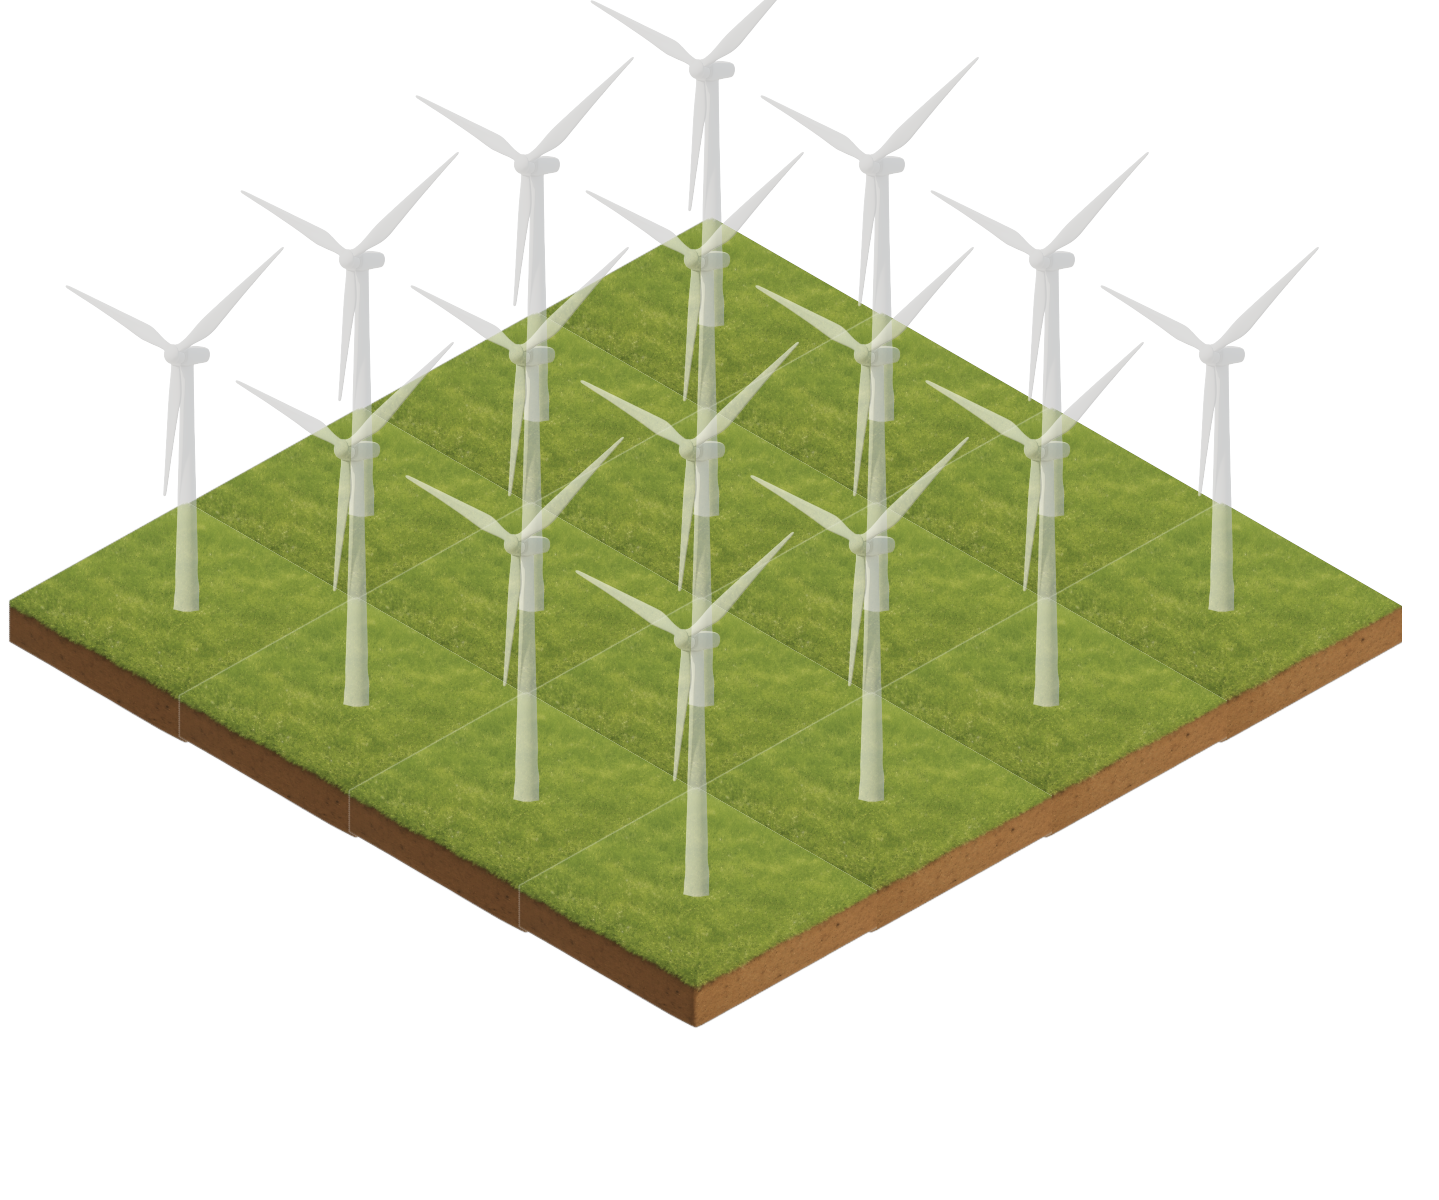
\includegraphics[width=\linewidth]{grid_4x4_inicial.png}\\[2pt]
      \small Estado inicial em superposição (4x4).
    \end{column}
  \end{columns}
\end{frame}

\begin{frame}{Layouts (2x3) e exemplo}
  \begin{columns}
    \begin{column}{0.45\textwidth}
      \centering
      % Substitua pelo arquivo mais recente gerado em images/
      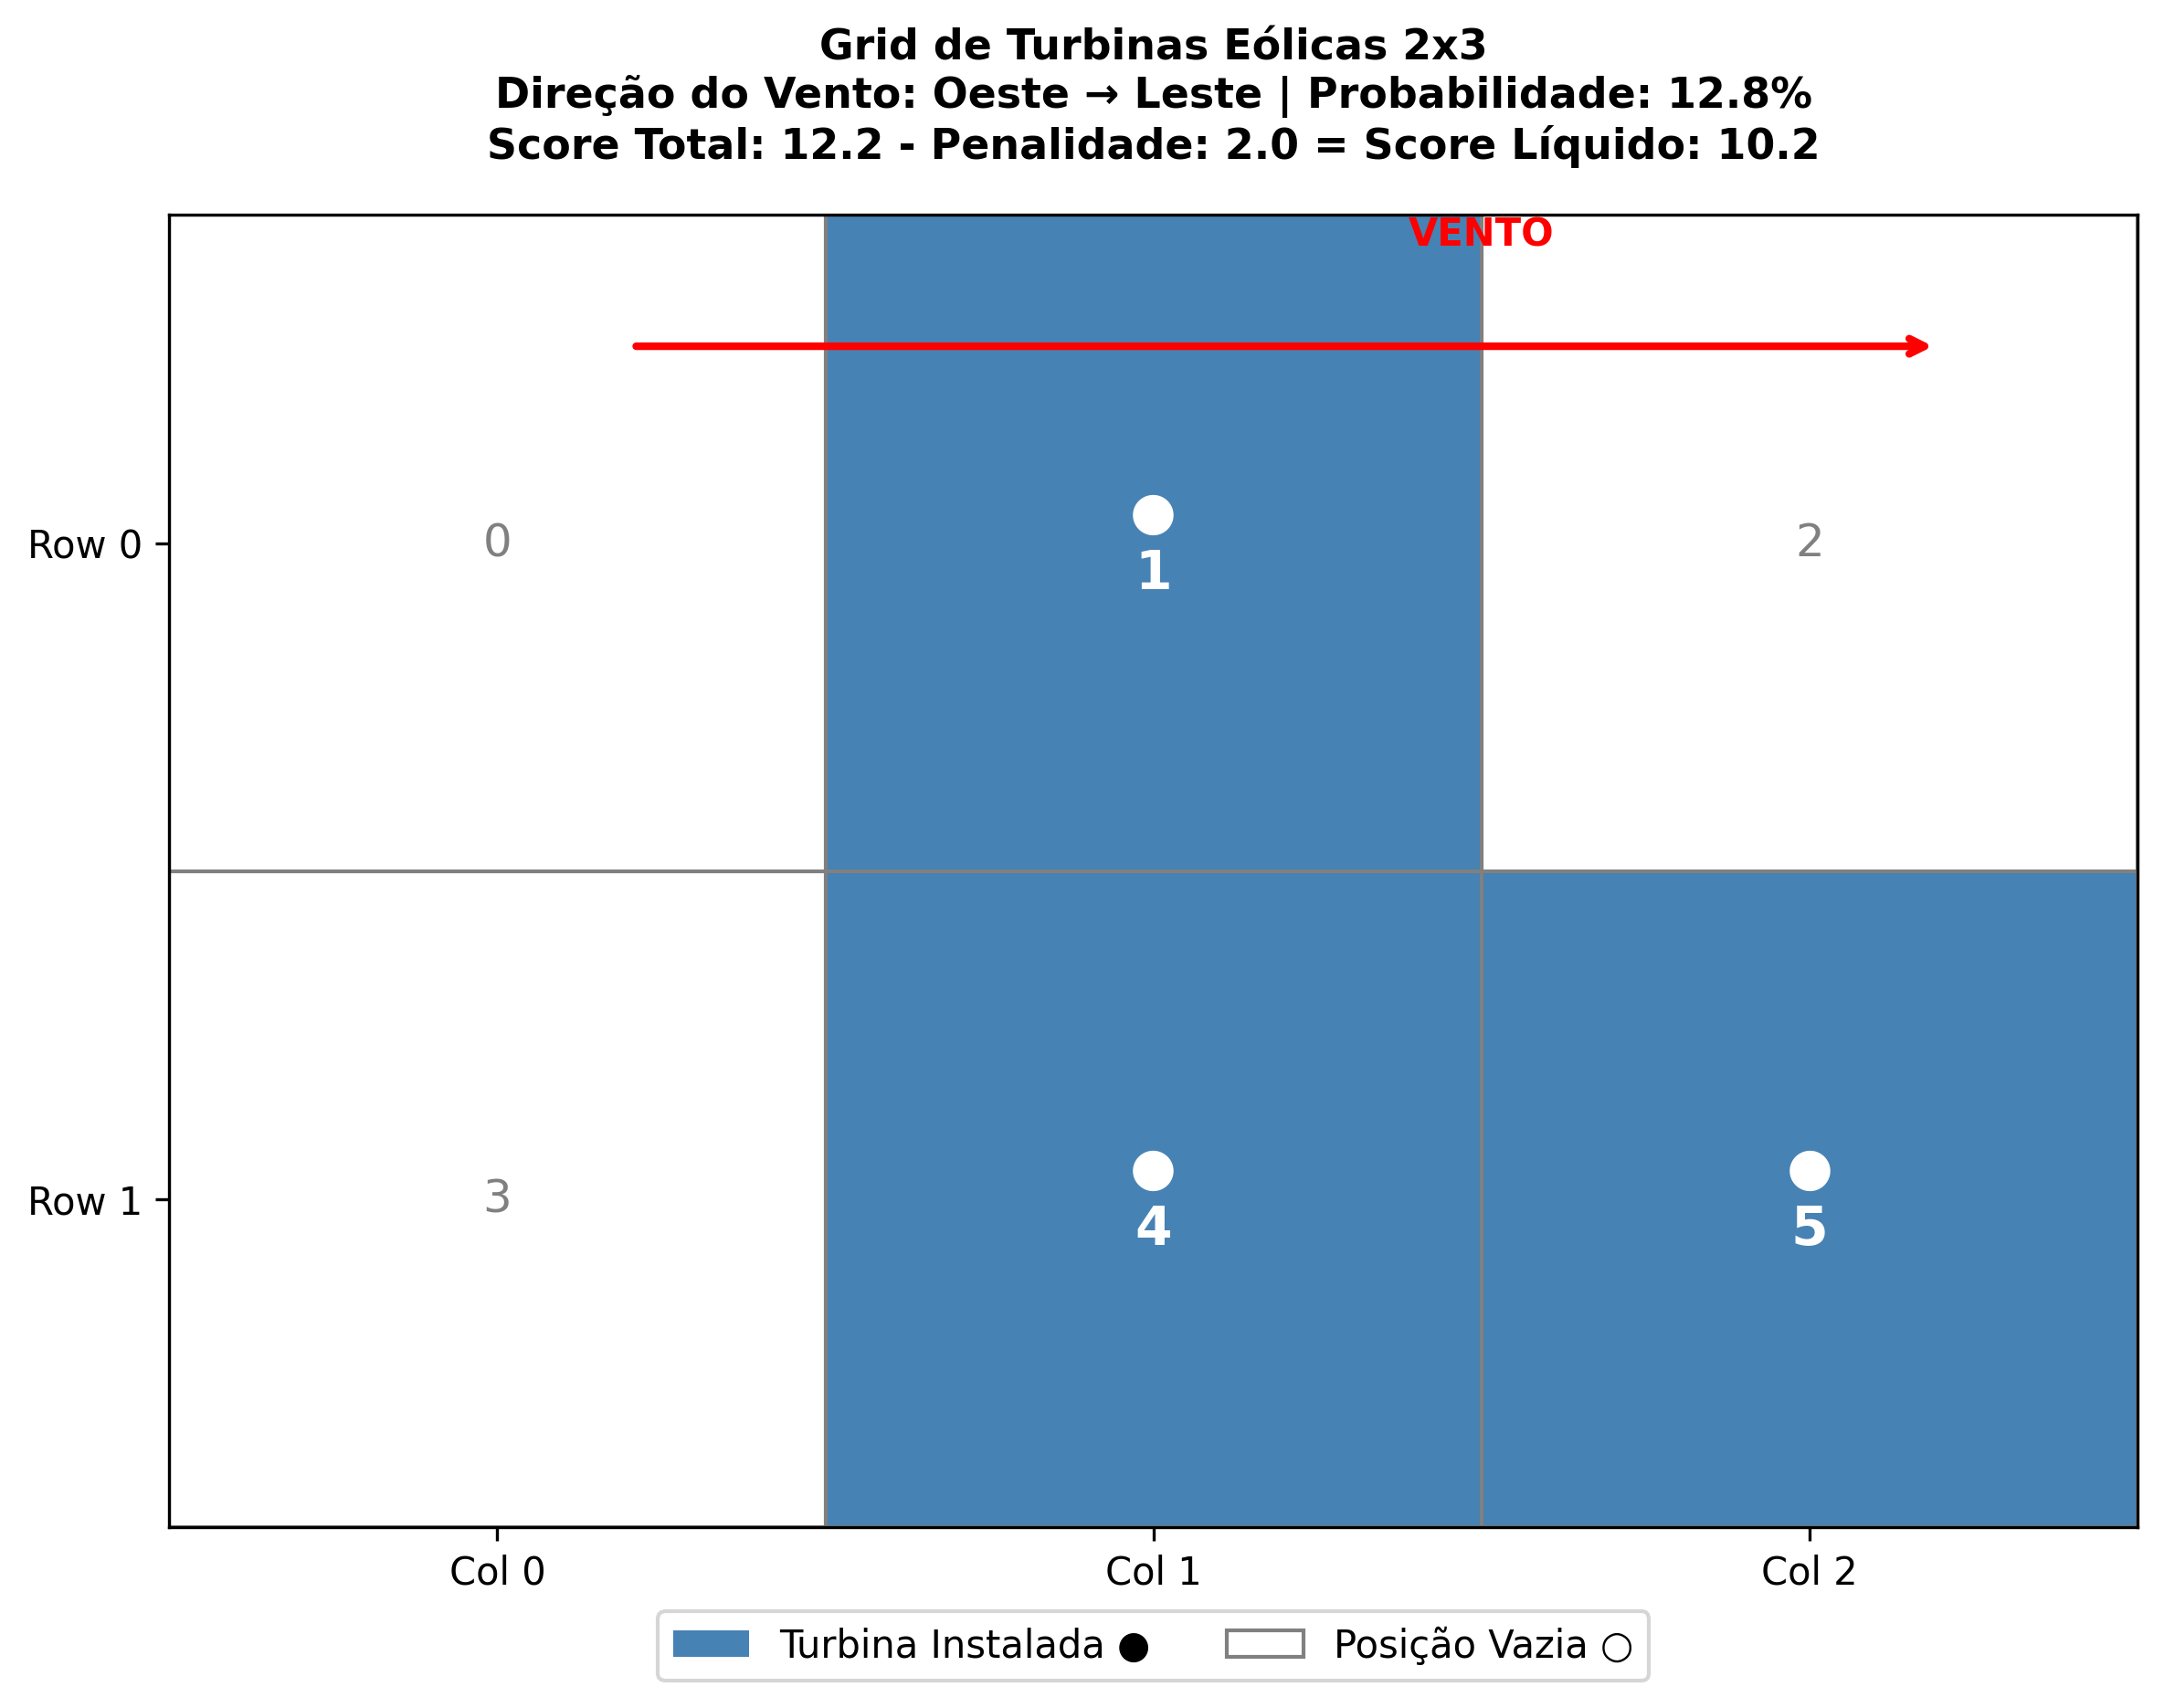
\includegraphics[width=\linewidth]{grid_visualization_default_2x3_3turbinas_20250810_144135.png}
      \\ \small Visualização do layout (2x3) \textemdash{} execução A
    \end{column}
    \begin{column}{0.48\textwidth}
      \centering
      \includegraphics[width=\linewidth]{grid_visualization_default_2x3_3turbinas_20250810_144138.png}
      \\ \small Visualização do layout (2x3) \textemdash{} execução B
    \end{column}
  \end{columns}
\end{frame}

\begin{frame}{Layout otimizado (4x4) e custos}
  \centering
  % Exemplo sem espaços no nome do arquivo
  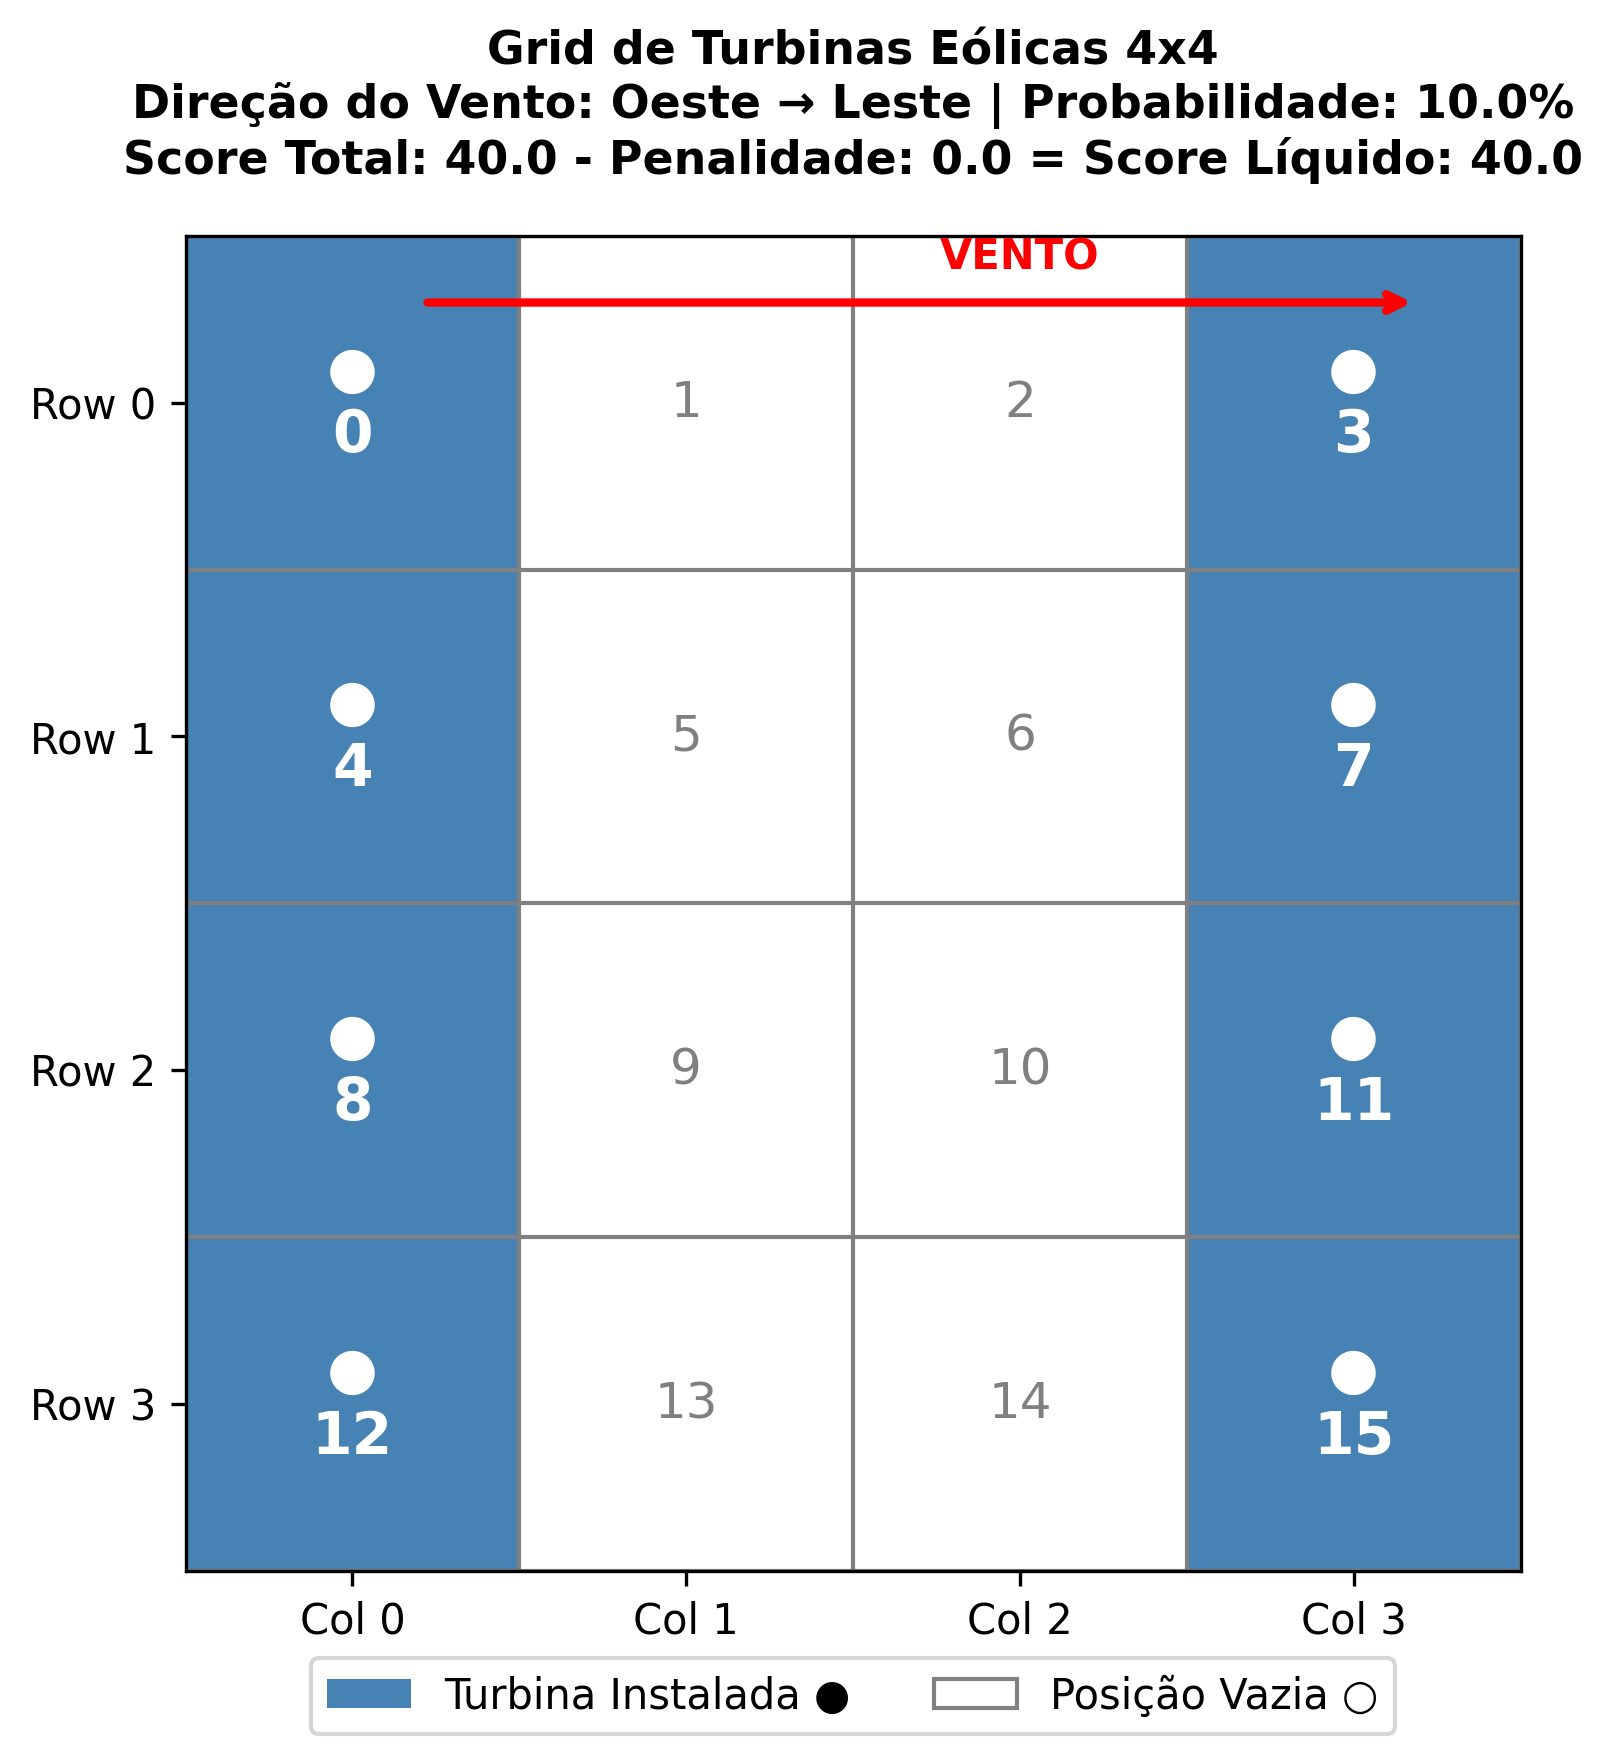
\includegraphics[width=0.78\linewidth]{grid_visualization_4x4_4x4_8turbinas_20250810_124433.png}
  \\[4pt]
  \small Custo final e conflitos mínimos sob penalidades da configuração.
\end{frame}

\begin{frame}{Discussão}
  \begin{itemize}
    \item Soluções plausíveis em grades pequenas; sensíveis à escolha de pesos e limiares.
    \item \textbf{Trade-off} entre qualidade e tempo de execução conforme $p$ e avaliações.
    \item Escalabilidade: crescimento do espaço de busca exige heurísticas/estruturas adicionais.
  \end{itemize}
\end{frame}

% ------------------------------------------------------------------
% 5) Conclusões e Próximos Passos
% ------------------------------------------------------------------
\section{Conclusões e próximos passos}

\begin{frame}{Conclusões}
  \begin{itemize}
    \item QAOA viabiliza formulação híbrida para o layout de turbinas com esteiras simplificadas.
    \item Pipeline reproduzível com \texttt{config*.json} e salvamento automático de resultados.
  \end{itemize}
\end{frame}

\begin{frame}{Trabalhos futuros}
  \begin{itemize}
    \item Refinar modelo de esteiras e calibração de penalidades.
    \item Estudo de ruído e execução em \textit{backends} reais.
    \item Técnicas de \textit{warm-start}, \textit{layerwise} e ajustes de otimizadores.
  \end{itemize}
\end{frame}

% ------------------------------------------------------------------
% 6) Demonstração rápida (CLI)
% ------------------------------------------------------------------
\section{Demonstração}

% ------------------------------------------------------------------
% 7) Agradecimentos e Referências
% ------------------------------------------------------------------
\section{Agradecimentos e referências}

\begin{frame}{Agradecimentos}
  \begin{itemize}
    \item Apoio institucional (UFERSA).
    \item Comunidade Qiskit e contribuidores do projeto.
  \end{itemize}
\end{frame}

\begin{frame}{Referências}
  \footnotesize
  \begin{itemize}
    \item Farhi, Goldstone, Gutmann. A Quantum Approximate Optimization Algorithm (2014).
    \item Documentação Qiskit e tutoriais de variational algorithms.
    \item Revisões sobre modelos de esteiras (ex.: Jensen/Park) e layout eólico.
  \end{itemize}
\end{frame}

\begin{frame}{Contato e repositório}
  \begin{itemize}
    \item Repositório: \url{https://github.com/}
    \item Contato: [e-mail/QR code]
  \end{itemize}
\end{frame}

\end{document}
